\chapter{Redactare și probleme de construcții}






\section{Redactarea în analiză: de la desen la demonstrație}

\subsection{Cum se redactează o soluție, în general}

Înainte de orice specific de analiză, regulile care valorează puncte la \emph{orice} probă:

\begin{enumerate}[leftmargin=*, itemsep=2pt]
\item \textbf{Anunță planul și structura.} Prima frază spune ce vei demonstra și, ideal, cum („Arătăm că $f$ e constantă, în doi pași: întâi că e periodică cu perioade oricât de mici, apoi concluzia prin continuitate.''). Pașii lungi devin \emph{leme cu nume} --- corectorul punctează pe schema ta, nu pe a lui.
\item \textbf{Fiecare afirmație are o acoperire:} un calcul afișat sau o teoremă \emph{numită, cu ipotezele verificate explicit} („$f$ e continuă pe $[0,1]$ ca sumă de funcții continue, deci prin Weierstrass își atinge maximul''). „Se vede că'' și „evident'' sunt puncte pierdute --- dacă e evident, demonstrația e scurtă; scrie-o.
\item \textbf{Obiectele se introduc înainte de a fi folosite}, cu cuantificatorul lor corect: „Fie $\varepsilon>0$ arbitrar'', „\emph{există} $N$ astfel încât...'', „\emph{alegem} $\delta=\min(\delta_1,\delta_2)$''. Ordinea cuantificatorilor e conținut matematic, nu stil --- inversarea lor e diferența dintre continuitate și continuitate uniformă.
\item \textbf{Notațiile: o dată definite, niciodată reciclate.} Nu folosi $n$ și pentru rangul șirului și pentru gradul polinomului; nu redefini $c$-ul de la teorema de medie în alt $c$ trei rânduri mai jos.
\item \textbf{Cazurile se epuizează la vedere.} Enumeră-le („Cazul 1: $f'(x_0)>0$...''), și scrie „cazul 2 e simetric, înlocuind $\max$ cu $\min$'' \emph{doar} dacă simetria e reală și verificabilă în 10 secunde.
\item \textbf{La „determinați...'': două jumătăți obligatorii.} \emph{Verificarea} (obiectele găsite chiar satisfac condiția --- calcul explicit) și \emph{clasificarea} (nu există altele). Baremul le desparte aproape întotdeauna; a preda doar ghicitul verificat înseamnă a preda jumătate de problemă.
\item \textbf{Ciorna nu intră în lucrare.} Drumul prin care ai găsit soluția (desene, cazuri mici, euristici, ecuația-busolă de la asimptotice) rămâne pe ciornă; pe curat intră doar lanțul logic, în ordinea logică --- nu în ordinea descoperirii. O pagină completă bate trei pagini de căutări.
\item \textbf{Ultimele 5 minute: auditul.} Capete de interval și ipoteze de tip închis/deschis, cazuri degenerate ($n=1$, funcția constantă, $a=b$), constante de integrare, semnele la ridicări la pătrat --- exact locurile din listele de capcane de mai jos.
\end{enumerate}

\subsection{Metoda grafică: de la desen la demonstrație}

Multe probleme de analiză se \emph{rezolvă} așa: faci un grafic, interpretezi grafic condiția din enunț, „vezi'' soluția pe desen, apoi te întorci la problemă. Este metoda corectă de \textbf{găsit} soluția --- graficul e cel mai rapid generator de intuiție din analiză. Dar aici e și capcana: \textbf{o soluție redactată pe desen primește, de obicei, cel mult 2 puncte din 7.} Graficul este schelă, nu demonstrație: comisia nu punctează „se vede din figură'', ci lanțul de teoreme care înlocuiește figura.

Fluxul corect de lucru este deci în \emph{două treceri}:
\begin{enumerate}[leftmargin=*, itemsep=2pt]
\item \textbf{Trecerea de descoperire (pe ciornă):} desenezi, interpretezi geometric condiția (o inegalitate = o poziție relativă de grafice; o ecuație = o intersecție; o medie = o arie sau o pantă), ghicești configurația și soluția.
\item \textbf{Trecerea de redactare (pe curat):} traduci \emph{fiecare} afirmație vizuală într-un enunț de teoremă. Dicționarul standard: „graficul urcă'' $\to$ monotonie demonstrată din semnul derivatei (pe \emph{interval}!); „graficele se intersectează'' $\to$ Cauchy--Bolzano/Darboux pe o funcție diferență, cu semnele de la capete calculate explicit; „graficul stă deasupra tangentei/coardei'' $\to$ convexitate, cu inegalitatea tangentei sau lema pantelor citată; „se apropie de...'' $\to$ limită cu $\varepsilon$ sau încadrare; „aria/panta medie'' $\to$ teoremă de medie sau Lagrange, cu ipotezele verificate. Dacă o propoziție din redactare nu are în spate o teoremă din fișă sau un calcul, ea nu există pentru corector.
\end{enumerate}

\subsection*{Exemplu}

\emph{Să se determine funcțiile $f:\mathbb{R}\to\mathbb{R}$ derivabile, cu derivata continuă, astfel încât}
\[
f(x)=\max\big(f'(x),\ x+1\big),\qquad\forall x\in\mathbb{R}.
\]

\emph{Trecerea 1 (descoperirea, pe desen).}

\smallskip
\noindent\textbf{Observație cheie.} Din continuitatea lui $f'$: dacă $f'(x_0)>x_0+1$ strict, atunci $f'(x)>x+1$ pe un întreg interval în jurul lui $x_0$ (și invers). Deci pe fiecare interval maximal avem exact una din situații:
\begin{itemize}[nosep,leftmargin=1.8em]
\item $f'(x)>x+1$: atunci $f(x)=f'(x)$, deci $f'=f$, adică $f(x)=Ce^x$ pe acel interval;
\item $f'(x)\le x+1$: atunci $f(x)=x+1$, deci $f'(x)=1$, iar condiția $1\le x+1$ cere $x\ge0$ (cu inegalitate strictă $f'(x)<x+1$ exact pentru $x>0$); un tronson liniar poate exista deci doar în $[0,\infty)$.
\end{itemize}

\noindent Altfel spus, $f$ este \textbf{pe bucăți}: alternează între tronsoane exponențiale $Ce^x$ și tronsoane liniare $x+1$.

\smallskip
\noindent\textbf{Ce s-ar putea întâmpla?} Graficul de mai jos arată o funcție care alternează liniar $\to$ exponențial $\to$ liniar $\to$ exponențial $\to$ liniar. Întrebarea: pot aceste bucăți să se „lipească'' consistent?

\begin{figure}[h]
\centering
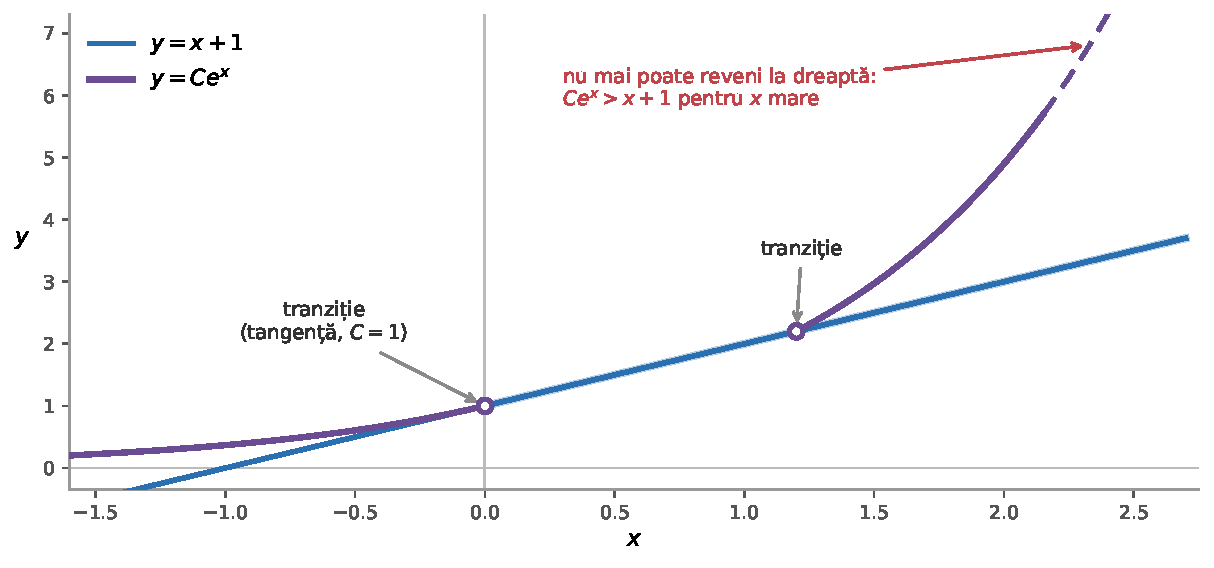
\includegraphics[width=0.86\textwidth]{grafic_p12_nou.pdf}
\caption*{\small\textit{O funcție pe bucăți candidat: alternează între $y=x+1$ (albastru) și $Ce^x$ (mov). Săgețile arată punctele de tranziție. Cheia: odată ce exponențiala depășește dreapta, nu mai poate reveni la ea, deoarece $Ce^x > x+1$ pentru $x$ suficient de mare.}}
\end{figure}

\noindent\textbf{De ce nu funcționează alternarea?} La o tranziție de la exponențial $\to$ liniar trebuie ca $Ce^{x_1} = x_1+1$ și $Ce^{x_1}=1$ (lipire $C^1$), adică tocmai tangența $e^{x_1}\ge x_1+1$, cu egalitate. Singura soluție: $C=1$, $x_1=0$. Dar pentru $x>0$, $e^x > x+1$ strict, deci exponențiala nu mai coboară niciodată la dreaptă. Orice tranziție după $x=0$ este imposibilă. Rămân doar: familia $Ce^x$ (cu $C\ge1$, ca să fie mereu $\ge x+1$) și soluția lipită o singură dată în $x=0$.

\medskip

\emph{Trecerea 2 (redactarea).} Fie $U=\{x:\ f'(x)<x+1\}$ --- mulțime \emph{deschisă}, fiindcă $f'$ e \textbf{continuă} (aici se folosește ipoteza!).

\emph{Pe $U$:} $f(x)=\max(f'(x),x+1)=x+1$, deci, $U$ fiind deschisă, $f'(x)=1$ pe $U$. Dar atunci condiția de apartenență $f'(x)<x+1$ devine $1<x+1$, adică $x>0$: așadar $U\subseteq(0,\infty)$.

\emph{Cazul $U=\varnothing$:} atunci $f'(x)\ge x+1$ peste tot, deci $f(x)=f'(x)$ pentru orice $x$. Ecuația $f'=f$ dă $f(x)=Ce^x$ (prin funcția auxiliară $f(x)e^{-x}$, ca în secțiunea de ecuații diferențiale). Rămâne constrângerea $Ce^x\ge x+1$ pentru orice $x$: pentru $C\le0$ pică în $x=0$; pentru $C>0$, minimul funcției $Ce^x-x-1$ se atinge în $x=-\ln C$ și valorează $\ln C$, deci constrângerea e echivalentă cu $C\ge1$. Obținem familia $f(x)=Ce^x$, $C\ge1$.

\emph{Cazul $U\neq\varnothing$:} fie $(a,b)$ o componentă a lui $U$, cu $0\le a<b\le\infty$. Pe $(a,b)$, $f'\equiv1$; prin continuitatea lui $f'$, $f'(a)=1$. Dar $a\notin U$, deci $f'(a)\ge a+1$, adică $1\ge a+1$, deci $a\le0$: combinat cu $a\ge0$, rezultă $a=0$. Dacă $b<\infty$: la fel $f'(b)=1\ge b+1$, deci $b\le0$ --- contradicție cu $b>0$. Așadar $U=(0,\infty)$, și $f(x)=x+1$ pe $[0,\infty)$ (cu $f(0)=1$ din continuitate). Pe $(-\infty,0]$, complementara lui $U$, avem $f=f'$ (ca mai sus), deci $f(x)=Ce^x$ acolo; $f(0)=1$ dă $C=1$. Verificări finale: lipirea e de clasă $C^1$ ($f'(0-)=e^0=1=f'(0+)$), iar pe $(-\infty,0)$ constrângerea $f'(x)=e^x\ge x+1$ e clasică. \hfill$\blacksquare$

\textbf{Răspuns:} $f(x)=Ce^x$ cu $C\ge1$, \emph{sau} $f(x)=\begin{cases}e^x,&x\le0\\ x+1,&x\ge0.\end{cases}$

\emph{Ce a cumpărat redactarea:} desenul a \emph{ghicit} ambele familii, dar numai argumentul cu mulțimea deschisă $U$ demonstrează că \textbf{nu există altele} --- exact partea invizibilă pe grafic. De remarcat și dicționarul la lucru: „tangenta lui $e^x$ la dreaptă'' $\to$ minimul lui $Ce^x-x-1$ calculat cu derivata; „lipirea merge'' $\to$ verificarea explicită $C^1$; „de la $0$ încolo doar dreapta'' $\to$ argumentul cu capetele componentelor lui $U$.

\subsection{Capcane frecvente (clasa a XI-a)}
\begin{enumerate}[leftmargin=*, itemsep=2pt]
\item Trecerea la limită în recurență cere \emph{mai întâi} demonstrarea convergenței; $\ell=f(\ell)$ singură nu dovedește nimic.
\item Lagrange/Rolle cer continuitate pe intervalul \emph{închis} și derivabilitate pe cel \emph{deschis} --- de verificat explicit ipotezele.
\item Consecințele lui Lagrange (monotonie din semnul derivatei) sunt valabile doar pe \emph{intervale}, nu pe reuniuni de intervale (ex. $-1/x$ are derivată pozitivă pe $\mathbb{R}^*$ dar nu e crescătoare pe $\mathbb{R}^*$).
\item L'Hôpital: de verificat forma nedeterminată și existența limitei raportului derivatelor; implicația nu se inversează.
\item Darboux nu implică continuitate; continuitate implică Darboux.
\item $a_{n+1}-a_n\to 0$ nu implică convergența; $\frac{a_{n+1}}{a_n}\to 1$ nu decide nimic.
\item Punctele de extrem pot fi și în capetele domeniului sau în puncte de nederivabilitate --- Fermat acoperă doar punctele interioare cu derivată.
\item La limite cu $\limsup/\liminf$ sau subșiruri: convergența pe $(x_{2n})$ și $(x_{2n+1})$ trebuie să dea \emph{aceeași} limită.
\end{enumerate}

\subsection{Capcane la integrale (clasa a XII-a)}
\begin{enumerate}[leftmargin=*, itemsep=2pt]
\item „Continuă $\iff$ are primitive'' e fals în ambele rafinări: continuitatea e suficientă dar nu necesară; Darboux e necesară dar nu suficientă.
\item Leibniz--Newton cere ca $G$ să fie primitivă pe \emph{tot} intervalul --- atenție la primitive „pe bucăți'' cu constante nepotrivite la lipire (clasic la $\int\frac{dx}{2+\cos x}$ cu substituția $t=\operatorname{tg}\frac x2$, discontinuă în $\pi$).
\item La schimbarea de variabilă pentru integrale definite se schimbă și capetele; $u$ trebuie să fie derivabilă cu derivata continuă pe intervalul de integrare.
\item $\int_a^b f=0$ nu implică $f\equiv0$ fără ipotezele $f\ge0$ \emph{și} $f$ continuă.
\item Integrabilitatea Riemann cere mărginire; $\int_0^1\frac{dx}{\sqrt x}$ este integrală \emph{improprie}, nu Riemann obișnuită --- se tratează prin limită.
\item În sume Riemann, funcția trebuie să fie integrabilă pe intervalul închis; singularitățile la capete (ca la $x^{-\alpha}$) cer argument suplimentar de trunchiere.
\end{enumerate}

\section{Construcții: ce funcții să încerci}

\emph{Notă:} secțiunea stă la început fiindcă e o \emph{atitudine}, nu un capitol --- se folosește peste tot. Exemplele ei invocă noțiuni tratate riguros mai târziu (derivate, ecuații diferențiale, lipiri pe $\mathbb{Q}$, integrale improprii); la prima citire se pot sări demonstrațiile, reținând reflexele.

Problemele de construcții la ONM sunt, de multe ori, de tipul \emph{„demonstrați că există o funcție cu proprietățile...''} sau \emph{„dați un exemplu de funcție care...''}. Ideea principală: să recunoști rapid \textbf{ce formă de funcție are șanse mari să funcționeze}, apoi să determini parametrii prin calcul direct.

\subsection{Principii generale de construcție}

Problemele de construcție arată la fel în toate ramurile --- combinatorică, teoria numerelor, analiză --- și au un folclor comun de strategii (adaptat aici după materialul „Olympiad Constructions'' al lui Cody Johnson și literatura de combinatorică olimpică):

\begin{enumerate}[leftmargin=*, itemsep=2pt]
\item \textbf{Cazuri mici, întotdeauna primele.} Rezolvă problema pentru $n=1,2,3,4$: cazurile mici îți ghicesc răspunsul (minimul/maximul, forma) și, mai important, îți arată \emph{tiparul} după care se asamblează construcția generală. Echivalentul în analiză: încearcă întâi pe exemplele-jucărie din catalog.
\item \textbf{Construcție prin inducție/asamblare.} Dintr-o construcție de mărime $n$ se fabrică des una de mărime $n+1$ sau $2n$ (dublezi, lipești, adaugi o piesă). În analiză: lipirea funcțiilor pe bucăți ($e^x$ cu $x+1$ la ONM 1994), șirurile de funcții definite recursiv.
\item \textbf{Întâi demonstrează, apoi caută: îngustarea prin restricții.} Înainte de a căuta orbește, demonstrează \emph{proprietăți obligatorii} ale oricărei soluții (în analiză: semne, monotonii, valori forțate în puncte). Fiecare restricție taie din spațiul de căutare --- și de multe ori restricțiile, cumulate, \emph{dictează} construcția. E exact „structura ghicește'' din secțiunile noastre: la $(f')^2+1=f$, compararea gradelor a decis totul înainte de orice încercare.
\item \textbf{La „demonstrați sau infirmați'': atacă serios varianta NU.} Încearcă cu adevărat să demonstrezi imposibilitatea; \emph{locul precis unde argumentul tău eșuează} e harta către construcție --- acolo e libertatea pe care o construcție trebuie s-o exploateze. Și disciplina de concurs: dacă în prima jumătate a timpului n-ai demonstrat „da'', petrece a doua jumătate pe „nu'' --- fără să oscilezi.
\item \textbf{Principiul simplității.} Dacă există o construcție, aproape sigur există una din \emph{piese simple}: mișcări elementare, blocuri repetate, funcții din catalog. Nu căuta obiecte exotice înainte de a epuiza combinațiile banale --- morala tuturor exemplelor din fișă, unde răspunsurile au fost $e^x$, $|x|$, Dirichlet, $\sqrt{x^2+\varepsilon}$, niciodată ceva nemaivăzut.
\end{enumerate}

Restul secțiunii aplică aceste principii la specificul analizei: ce \emph{familii de funcții} joacă rolul „pieselor simple''.

\begin{tehbox}{Reflexul 1: la ecuații funcționale sau diferențiale, încearcă întâi un polinom}

Primul reflex este să presupui că funcția e polinom și să vezi \emph{ce grad ar trebui să aibă}: compararea gradelor spune foarte repede dacă există vreo șansă. Regulile de grad: derivarea scade gradul cu $1$; ridicarea la pătrat îl dublează; compunerea le înmulțește.

\textbf{Exemplu.} Să se construiască $f$ cu $\big(f'(x)\big)^2+1=f(x)$ pentru orice $x$.

\emph{Pasul 1 (gradul).} Dacă $f$ e polinom de grad $n$: $f'$ are grad $n-1$, deci $(f')^2$ are grad $2(n-1)$. Egalitatea gradelor cere $2(n-1)=n$, adică $n=2$. Încercăm $f(x)=ax^2+bx+c$.

\emph{Pasul 2 (calcul direct).} $f'(x)=2ax+b$, deci
\[
(2ax+b)^2+1=ax^2+bx+c
\quad\Longleftrightarrow\quad
4a^2x^2+4abx+b^2+1=ax^2+bx+c,
\]
și identificarea coeficienților dă sistemul $4a^2=a$, $4ab=b$, $b^2+1=c$.

\emph{Pasul 3 (rezolvarea).} Din prima: $a=0$ (pierde gradul 2) sau $a=\frac14$. Pentru $a=\frac14$, a doua ecuație devine $b\cdot0=0$, deci $b$ e \emph{arbitrar}, iar $c=b^2+1$:
\[
\boxed{\ f(x)=\frac{x^2}{4}+bx+b^2+1,\qquad b\in\mathbb{R}.\ }
\]
Verificare: $f'(x)=\frac x2+b$, $\big(\frac x2+b\big)^2+1=\frac{x^2}4+bx+b^2+1=f(x)$. \checkmark

\end{tehbox}

\subsection{Reflexul 2: condiția $f>0$ pe tot domeniul}

Când enunțul cere $f(x)>0$ pentru orice $x$ din domeniu (de obicei $(0,\infty)$), formele naturale de testat sunt
\[
f(x)=c_2\,x^{c_1}\qquad\text{și}\qquad f(x)=b\cdot a^{x},
\]
cu $c_2,b>0$ --- puterile și exponențialele sunt pozitivele „canonice'' și se comportă perfect la înmulțiri, compuneri și derivări (rămân în aceeași familie). Nu întâmplător: acestea sunt exact soluțiile ecuațiilor funcționale clasice (secțiunea de ecuații Cauchy), deci orice condiție cu structură multiplicativă le va selecta.

\subsection{Reflexul 3: discontinuități controlate --- funcții de tip Dirichlet}

Când trebuie construită o funcție cu un număr \emph{controlat} de puncte de discontinuitate sau de nederivabilitate, ideea standard este definirea diferită pe $\mathbb{Q}$ și pe $\mathbb{R}\setminus\mathbb{Q}$. Instrumentul teoretic e deja în fișă (subsecțiunea „Funcții definite prin cazuri pe $\mathbb{Q}$ și $\mathbb{R}\setminus\mathbb{Q}$''): pentru $g,h$ continue, funcția lipită e \textbf{continuă exact în punctele unde $g(x)=h(x)$}, și derivabilă exact unde ramurile se ating cu tot cu derivate. Construcția devine astfel o \emph{ecuație}: vrei discontinuitate exact pe o mulțime $S$? Alege ramuri care coincid exact pe complementara lui $S$.

\subsection{Reflexul 4: Ce funcții clasice care verifică ipoteza știu?}

Înainte de a inventa ceva complicat, pune-ți întrebarea: \emph{„ce exemplu cu proprietățile acestea știu deja?''} Subpunctele de tip „dați un exemplu / rezultă că...?'' de la olimpiadă se rezolvă aproape întotdeauna dintr-un catalog scurt, combinat cu mici ajustări (translații, înmulțiri cu constante, $x^2+\varepsilon$ în loc de $x^2$):

\begin{enumerate}[leftmargin=*, itemsep=2pt]
\item \textbf{Dirichlet} $\mathbf{1}_{\mathbb{Q}}$ --- discontinuă peste tot; $x\cdot\mathbf{1}_{\mathbb{Q}}$ --- continuă doar în $0$; $x$ pe $\mathbb{Q}$, $x+1$ în rest --- discontinuă peste tot dar cu limite „pe ramuri''.
\item $|x|$ --- continuă, nederivabilă într-un punct; $\sqrt{x^2+\varepsilon}$ --- neteda care o aproximează.
\item $\sin\frac1x$ --- mărginită fără limită în $0$; $x\sin\frac1x$ --- continuă, nederivabilă în $0$; $x^2\sin\frac1x$ --- derivabilă cu derivata discontinuă.
\item $x^3$ --- strict crescătoare cu derivata nulă într-un punct; $x+2\sin x$ --- derivată care schimbă semnul de infinite ori, dar funcția $\to\infty$.
\end{enumerate}

Morala: la punctele b) de tip „rezultă că...?'', răspunsul „nu'' se demonstrează cu un membru al catalogului, ajustat minimal.

\subsection*{Exemplu}

\emph{Fie $f:\mathbb{R}\to\mathbb{R}$ pentru care există o funcție derivabilă $g:\mathbb{R}\to\mathbb{R}$ și un șir $(a_n)$ de numere strict pozitive, convergent la $0$, astfel încât}
\[
g'(x)=\lim_{n\to\infty}\frac{f(x+a_n)-f(x)}{a_n}\qquad\forall x\in\mathbb{R}.
\]
\emph{a) Dați un exemplu de astfel de $f$ care nu e derivabilă în niciun punct.}

\emph{Soluție.} Gândim simplu: ne trebuie o funcție nederivabilă peste tot --- primul candidat din catalog e Dirichlet, $f=\mathbf{1}_{\mathbb{Q}}$. Verificăm că merge cu $a_n=\frac1n$: dacă $x\in\mathbb{Q}$, atunci $x+\frac1n\in\mathbb{Q}$; dacă $x\notin\mathbb{Q}$, atunci $x+\frac1n\notin\mathbb{Q}$ --- adunarea unui rațional \emph{păstrează clasa}. Deci
\[
f\Big(x+\frac1n\Big)=f(x)\quad\forall x,n
\qquad\Longrightarrow\qquad
\frac{f(x+a_n)-f(x)}{a_n}=0\to0,
\]
așa că ipoteza e satisfăcută cu $g$ constantă ($g'\equiv0$). Iar $f$ e discontinuă în orice punct (ramurile constante $1$ și $0$ nu se ating nicăieri --- corolarul lipirii), deci nederivabilă peste tot. $\blacksquare$

\emph{De reținut:} toată soluția stă în alegerea șirului $a_n$ \emph{rațional} --- limita pe un șir particular nu vede structura fină a funcției. Exact acest fenomen face ca punctul b) al problemei (dacă $f$ e \emph{continuă}, atunci e derivabilă) să fie partea grea.

\subsection*{Exemplu: ONM 2026, etapa națională, clasa a XI-a, Problema 1b)}

\textbf{Enunț.} Fie $h:\mathbb{R}\to\mathbb{R}$ o funcție continuă și $(f_n)$, $(g_n)$ două șiruri de funcții derivabile cu proprietatea că $f_n(x)<h(x)<g_n(x)$ pentru orice $x\in\mathbb{R}$ și orice $n\in\mathbb{N}^*$, și că $g_n(x)-f_n(x)\to0$ pentru orice $x\in\mathbb{R}$. Este $h$ neapărat derivabilă?

\textbf{Răspuns: NU.}

Am participat la ONM 2026 și acesta a fost raționamentul meu la această problemă.

\emph{Cum se ghicește contraexemplul.} În timpul concursului am desenat un grafic. Condițiile problemei spun că $h$ e prinsă între două familii de funcții derivabile care o strivesc --- pe grafic asta înseamnă două „clești'' de curbe netede care coboară și urcă spre $h$ din ambele părți. Singura funcție continuă și nederivabilă pe care o știam era $h(x)=|x|$ --- are un colț în $0$, dar e altfel perfect inofensivă. Am desenat-o și am căutat cu ochii niște curbe derivabile, mai sus și mai jos, care să o strângă:

\begin{center}
\begin{tikzpicture}[scale=2.0, >=latex]
  % Axe
  \draw[->] (-1.30,0) -- (1.32,0) node[right] {$x$};
  \draw[->] (0,-0.50) -- (0,1.28) node[above] {$y$};
  \node[below left, font=\small] at (0,0) {$0$};

  % Curbe de sus -- violet, intrerupte
  \draw[onm!35, line width=0.85pt, dashed, domain=-1.28:1.28, samples=100]
    plot (\x, {sqrt(\x*\x + 1)});
  \draw[onm!65, line width=1pt, dashed, domain=-1.28:1.28, samples=100]
    plot (\x, {sqrt(\x*\x + 0.25)});
  \draw[onm, line width=1.3pt, dashed, domain=-1.28:1.28, samples=100]
    plot (\x, {sqrt(\x*\x + 0.04)});

  % Curbe de jos -- portocaliu, punctate, coboara sub 0
  \draw[ojm!35, line width=0.85pt, dotted, domain=-1.28:1.28, samples=100]
    plot (\x, {sqrt(\x*\x + 1) - 1.4142});
  \draw[ojm!65, line width=1pt, dotted, domain=-1.28:1.28, samples=100]
    plot (\x, {sqrt(\x*\x + 0.25) - 0.7071});
  \draw[ojm, line width=1.3pt, dotted, domain=-1.28:1.28, samples=100]
    plot (\x, {sqrt(\x*\x + 0.04) - 0.2828});

  % |x| -- linie groasa, desenata dupa curbe ca sa fie deasupra
  \draw[ink, line width=2.4pt, domain=-1.28:0, samples=2]
    plot (\x, {-\x});
  \draw[ink, line width=2.4pt, domain=0:1.28, samples=2]
    plot (\x, {\x});

  % Eticheta h(x) -- in interiorul graficului, la stanga
  \node[ink, font=\small\bfseries, fill=white, inner sep=1pt]
    at (-0.75, 0.88) {$h(x)=|x|$};

  % Punct de colt
  \filldraw[ink] (0,0) circle (0.030);
  \node[ink, above right, font=\small] at (0.05, 0.04) {colț};

  % Etichete sus/jos
  \node[onm, font=\scriptsize\itshape] at (0.60, 1.15) {sus};
  \node[ojm, font=\scriptsize\itshape] at (0.75, 0.55) {jos};
\end{tikzpicture}
\end{center}

Forma curbelor de deasupra mi-a sugerat imediat o hiperbolă netezită. Odată ales $h$ și observat că curbele seamănă cu $\sqrt{x^2+\varepsilon}$, am ales formal:

\textbf{Construcția.} Punem
\[
g_n(x)=\sqrt{x^2+\tfrac1n},\qquad f_n(x)=\sqrt{x^2+\tfrac1n}-\sqrt{\tfrac2n}.
\]
\emph{Derivabilitate:} $x^2+\frac1n>0$, deci ambele sunt $C^\infty$ pe $\mathbb{R}$.

\emph{Încadrarea $f_n<h<g_n$:} Inegalitatea $g_n>|x|$ e clară. Inegalitatea $f_n<|x|$ revine la $\sqrt{x^2+\frac1n}-\sqrt{\frac2n}<|x|$, adică (ridicând la pătrat, ambii membri nenegativi pentru $n$ mare):
\[
x^2+\frac1n < x^2+2|x|\sqrt{\tfrac2n}+\frac2n
\quad\Longleftrightarrow\quad
0 < 2|x|\sqrt{\tfrac2n}+\frac1n,
\]
adevărată pentru orice $x\in\mathbb{R}$.

\emph{Strângerea:} $g_n(x)-f_n(x)=\sqrt{\frac2n}\to0$ uniform.

Toate ipotezele sunt satisfăcute, dar $h=|x|$ nu e derivabilă în $0$. $\blacksquare$


